% TODO: Use British and not American English:
%    * s/artifact/artefact/
%    * Too many commas. Read about best practices.
% TODO: Proof read for common mistakes:
%    * exist vs exists.

\documentclass[12pt, a4paper]{article}

% Preamble

\usepackage[utf8]{inputenc}
\usepackage[english]{babel}
\usepackage[margin=1in]{geometry}
\usepackage[parfill]{parskip}
\usepackage[hidelinks]{hyperref}
\usepackage{graphicx}
\usepackage{listings}
\usepackage{latex/nasm/lang}
\usepackage{latex/nasm/style}
\bibliographystyle{ieeetr}

\title{Compositional Decompilation}
\author{Robin Eklind}
\date{2014-10-04}

% Document

\begin{document}

\maketitle

\begin{abstract}
TODO
\end{abstract}

\vfill

\begin{quote}
	\textit{``What we call chaos is just patterns we haven't recognized. What we call random is just patterns we can't decipher.''} - Chuck Palahniuk \cite{patterns_quote}.
\end{quote}

\pagebreak

% TODO: Remember to display the acknowledgements page.

%\textbf{Acknowledgements}

%My heartfelt gratitude goes to Janka Chlebíková for supervising this project and showing me the beauty of Theoretical Computer Science; your joyful enthusiasm is inspiring!

\pagebreak

\tableofcontents

\pagebreak

%%%%%%%%%%%%%%%%%%%%%%%%%%%%%%%%%%%%%%%%%%%%%%%%%%%%%%%%%%%%%%%%%%%%%%%%%%%%%%%%
% Introduction
%%%%%%%%%%%%%%%%%%%%%%%%%%%%%%%%%%%%%%%%%%%%%%%%%%%%%%%%%%%%%%%%%%%%%%%%%%%%%%%%

% === [ Introduction ] =========================================================

\section{Introduction}

A compiler is a piece of software which translates human readable high-level programming languages (e.g. C) to machine readable low-level languages (e.g. Assembly). In the usual flow of compilation, code is lowered through a set of transformations from a high-level to a low-level representation. The decompilation process (originally referred to as reverse compilation \cite{rev_comp}) moves in the opposite direction by lifting code from a low-level to a high-level representation.

As recognized by Edsger W. Dijkstra in his 1972 ACM Turing Lecture (an extract from which is presented in figure \ref{dijkstra_lecture}) one of the most powerful tools for solving complex problems in Computer Science is the use of abstractions and separation of concerns. This paper explores a compositional approach to decompilation which facilitates abstractions to create a pipeline of self-contained components. Since the components interact through language-agnostic interfaces (well-defined input and output) each individual component may be written in a variety of programming languages. Furthermore, for each component of the decompilation pipeline there may exist multiple implementations with their individual strengths and weaknesses. The end user (e.g. malware analyst, security researcher, reverse engineer, …) may select the components which solves their task at hand the best.

\begin{figure}[htbp]
	\begin{quote}
		\textit{``We all know that the only mental tool by means of which a very finite piece of reasoning can cover a myriad cases is called ``abstraction''; as a result the effective exploitation of his powers of abstraction must be regarded as one of the most vital activities of a competent programmer. In this connection it might be worthwhile to point out that the purpose of abstracting is not to be vague, but to create a new semantic level in which one can be absolutely precise. Of course I have tried to find a fundamental cause that would prevent our abstraction mechanisms from being sufficiently effective. But no matter how hard I tried, I did not find such a cause. As a result I tend to the assumption -- up till now not disproved by experience -- that by suitable application of our powers of abstraction, the intellectual effort needed to conceive or to understand a program need not grow more than proportional to program length.''} \cite{abstractions_quote}
	\end{quote}
	\caption{An extract from the ACM Turing Lecture given by Edsger W. Dijkstra in 1972.}
	\label{dijkstra_lecture}
\end{figure}

% TODO: Find a good place to write about the applications of decompilation.

% --- [ Project Aim and Objectives ] -------------------------------------------

\subsection{Project Aim and Objectives}

The aim of this project is to facilitate decompilation workflows using composition of language-agnostic decompilation passes; specifically the reconstruction of high-level control structures and, as a future ambition, expressions.

In order to achieve this aim, the author will:
\begin{enumerate}
	\item Review traditional decompilation techniques, including control flow analysis and data flow analysis. \label{decomp_research_obj}
	\item Critically evaluate a set of Intermediate Representations (IR), which describes low-, medium- and high-level language semantics, to identify one or more suitable for the decompilation pipeline. \label{ir_evaluation_obj}
	\item Analyze the formal grammar (language specification) of the IR to verify that it is unambiguous. If the grammar is ambiguous or if no formal grammar exists, produce a formal grammar. This objective is critical for language-independence, as the IR works as a bridge between different programming languages. \label{formal_ir_obj}
	\item Determine if any existing library for the IR satisfies our requirements; and if not develop one. The requirements would include a suitable in-memory representation, and support for on-disk file storage and arbitrary manipulations (inject, delete, etc) of the IR. \label{ir_lib_obj}
	\item Design and develop components which identify the structural patterns of high-level control structures using control flow analysis of the IR. \label{structure_lib_obj}
	\item Develop tools which perform one or more decompilation passes on a given IR. The tools will be reusable by other programming language environments as their input and output is specified by a formally defined IR. \label{reconstruct_tool_obj}
	\item As a future ambition, design and develop components which perform expression propagation using data flow analysis of the IR. \label{expression_lib_obj}
\end{enumerate}

% --- [ Deliverables ] ---------------------------------------------------------

\subsection{Deliverables}

% TODO: Add https://github.com/mewrev/decomp when it is created.

The source code and the report of this project have been released into the public domain \cite{cc0} and are made available at:
\begin{itemize}
	\item \url{https://github.com/mewlang/llvm}
	\item \url{https://github.com/mewpaper/decompilation}
\end{itemize}

% TODO: Specify the deliverables of the project after the development phase has finished. Use the text below as a basis.
%
% The following documents have been produced:
% * Project report; refer to objective 1 and 2.
% * Formal grammar for a subset of the LLVM IR language; refer to objective 3.
%
% The following system artifacts have been developed:
% * Library for interacting with LLVM IR; refer to objective 4.
% * Library for reconstructing high-level control structures from LLVM IR; refer to objective 5.
% * Tool for performing one or more decompilation passes on a given IR; refer to objective 6.

% --- [ Disposition ] ----------------------------------------------------------

\subsection{Disposition}

Lorem ipsum dolor sit amet, consectetur adipiscing elit, sed do eiusmod tempor incididunt ut labore et dolore magna aliqua.

%%%%%%%%%%%%%%%%%%%%%%%%%%%%%%%%%%%%%%%%%%%%%%%%%%%%%%%%%%%%%%%%%%%%%%%%%%%%%%%%
% Literature Review
%%%%%%%%%%%%%%%%%%%%%%%%%%%%%%%%%%%%%%%%%%%%%%%%%%%%%%%%%%%%%%%%%%%%%%%%%%%%%%%%

% === [ Literature Review ] ====================================================

\section{Literature Review}

Lorem ipsum dolor sit amet, consectetur adipiscing elit, sed do eiusmod tempor incididunt ut labore et dolore magna aliqua.

% --- [ The Anatomy of an Executable ] -----------------------------------------

\subsection{The Anatomy of an Executable}

The representation of executables, shared libraries and relocatable object code is standardized by a variety of file formats which provides encapsulation of assembly instructions and data. Two such formats are the Portable Executable (PE) file format and the Executable and Linkable Format (ELF), which are used by Windows and Linux respectively. Both of these formats partition executable code and data into sections and assign appropriate access permissions to each section, as summarized by table \ref{elf_sections}. In general no single section has both write and execute permissions as this could compromise the security of the system.

\begin{table}[htbp]
	\begin{center}
		\begin{tabular}{|l|l|l|}
			\hline
			Section name & Usage description & Access permissions \\
			\hline
			\texttt{.text} & Assembly instructions & \texttt{r-x} \\
			\texttt{.rodata} & Read-only data & \texttt{r--} \\
			\texttt{.data} & Data & \texttt{rw-} \\
			\texttt{.bss} & Uninitialized data & \texttt{rw-} \\
			\hline
		\end{tabular}
	\end{center}
	\caption{A summary of the most commonly used sections in ELF files. The \texttt{.text} section contains executable code while the \texttt{.rodata}, \texttt{.data} and \texttt{.bss} sections contains data in various forms.}
	\label{elf_sections}
\end{table}

To gain a better understanding of the anatomy of executables the remainder of this section describes the structure of ELF files and presents the dissection of a simple \textit{``hello world''} ELF executable, largely inspired by Eric Youngdale's article on \textit{The ELF Object File Format by Dissection} \cite{elf_dissection}. Although the ELF and PE file formats differs with regards to specific details, the general principles are applicable to both formats.

In general ELF files consists of a file header, zero or more program headers, zero or more section headers and data referred to by the program or section headers, as depicted in figure \ref{elf_structure}.

\begin{figure}[htbp]
	\begin{center}
		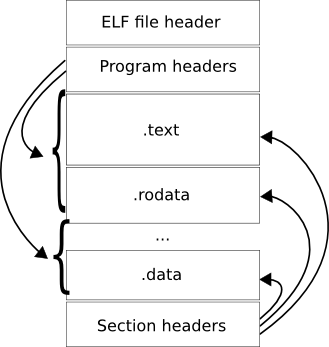
\includegraphics[width=0.5\textwidth]{inc/elf_structure.png}
		\caption{The basic structure of an ELF file. \textit{Image license:} CC BY-SA \cite{elf_structure_orig}}
		\label{elf_structure}
	\end{center}
\end{figure}

All ELF files starts with the four byte identifier \texttt{0x7F}, \texttt{'E'}, \texttt{'L'}, \texttt{'F'} which marks the beginning of the ELF file header. The ELF file header contains general information about a binary, such as its object file type (executable, relocatable or shared object), its assembly architecture (x86-64, ARM, …), the virtual address of its entry point which indicates the starting point of program execution, and the file offsets to the program and section headers.

Each program and section header describes a continuous segment or section of memory respectively. In general segments are used by the linker to load executables into memory with correct access permissions, while sections are used by the compiler to categorize data and instructions. Therefore the program headers are optional for relocatable and shared objects, while the section headers are optional for executables.

\begin{figure}[htbp]
	\begin{center}
		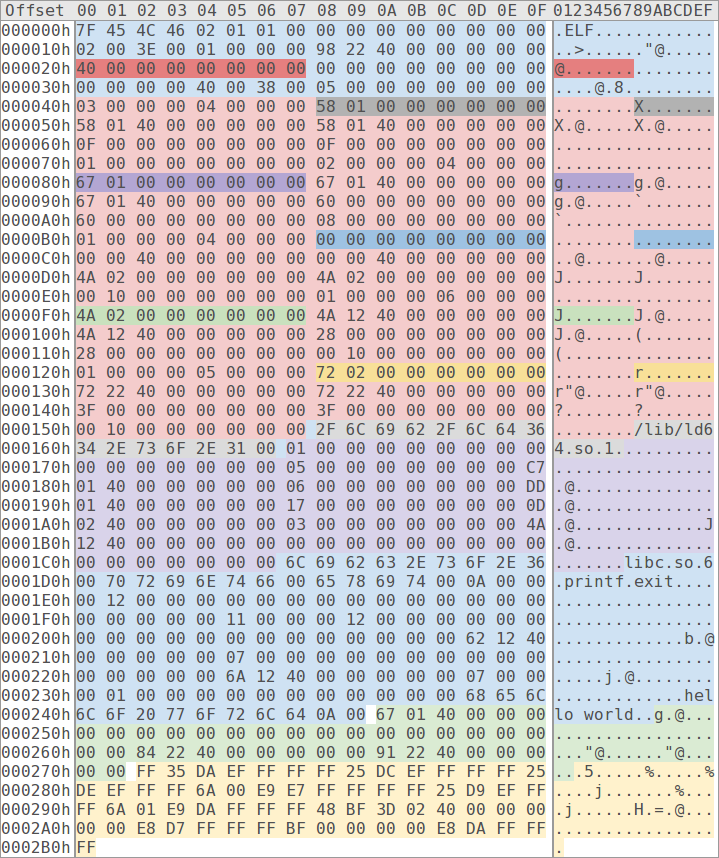
\includegraphics[width=\textwidth]{inc/elf_dissection.png}
		\caption{The entire contents of a simple \textit{``hello world''} ELF executable with color-coded file offsets, sections, segments and program headers, where each file offset is 8 bytes in width and colored using a darker shade of its corresponding segment, section or program header.}
		\label{elf_dissection}
	\end{center}
\end{figure}

To further investigate the structure of ELF files a simple 64-bit \textit{``hello world''} executable has been dissected and its content color-coded. Each file offset of the executable consists of 8 bytes and is denoted in figure \ref{elf_dissection} with a darker shade of the color used by its corresponding target segment, section or program header. Starting at the middle of the ELF file header, at offset \texttt{0x20}, is the file offset (red) to the program table (bright red). The program table contains five program headers which specify the size and file offsets of two sections and three segments, namely the \texttt{.interp} (gray) and the \texttt{.dynamic} (purple) sections, and a \textit{read-only} (blue), a \textit{read-write} (green) and a \textit{read-execute} (yellow) segment.

Several sections are contained within the three segments. The \textit{read-only} segment contains the following sections:

\begin{itemize}
	\item \texttt{.interp}: the interpreter, i.e. the linker
	\item \texttt{.dynamic}: array of dynamic entities
	\item \texttt{.dynstr}: dynamic string table
	\item \texttt{.dynsym}: dynamic symbol table
	\item \texttt{.rela.plt}: relocation entities of the PLT
	\item \texttt{.rodata}: read-only data section
\end{itemize}

The \textit{read-write} segment contains the following section:

\begin{itemize}
	\item \texttt{.got.plt}: Global Offset Table (GOT) of the PLT (henceforth referred to as the GOT as this executable only contains one such table)
\end{itemize}

And the \textit{read-execute} segment contains the following sections:

\begin{itemize}
	\item \texttt{.plt}: Procedure Linkage Table (PLT)
	\item \texttt{.text}: executable code section
\end{itemize}

Seven out of the nine sections contained within the executable are directly related to dynamic linking. The \texttt{.interp} section specifies the linker (in this case \textit{``/lib/ld64.so.1''}) and the \texttt{.dynamic} section an array of dynamic entities containing offsets and virtual addresses to relevant dynamic linking information. In this case the dynamic array specifies that \textit{``libc.so.6''} is a required library, and contains the virtual addresses to the \texttt{.dynstr}, \texttt{.dynsym}, \texttt{.rela.plt} and \texttt{.got.plt} sections. As noted, even a simple \textit{``hello world''} executable requires a large number of sections related to dynamic linking. Further analysis will reveal their relation to each other and describe their usage.

The dynamic string table contains the names of libraries (e.g. \textit{``libc.so.6''}) and identifiers (e.g. \textit{``printf''}) which are required for dynamic linking. Other sections refer to these strings using offsets into \texttt{.dynstr}. The dynamic symbol table declares an array of dynamic symbol entities, each specifying the name (e.g. offset to \textit{``printf''} in \texttt{.dynstr}) and binding information (local or global) of a dynamic symbol. Both the \texttt{.plt} and the \texttt{.rela.plt} sections refers to these dynamic symbols using array indicies. The \texttt{.rela.plt} section specifies the relocation entities of the PLT; more specifically it informs the linker of the virtual address to the \texttt{.printf} and \texttt{.exit} entities in the GOT.

Lets take a step back for a moment and reflect on how dynamic linking is accomplished on a Linux system by reviewing the assembly instructions of the executable \texttt{.text} and \texttt{.plt} sections as outlined in listing \ref{elf_text} and \ref{elf_plt} respectively.

\lstinputlisting[language=nasm,style=nasm,caption={The assembly instructions of the \texttt{.text} section.\label{elf_text}},xleftmargin=1cm,xrightmargin=1cm]{inc/elf_text.asm}

\lstinputlisting[language=nasm,style=nasm,caption={The assembly instructions of the \texttt{.plt} section.\label{elf_plt}},xleftmargin=1cm,xrightmargin=1cm]{inc/elf_plt.asm}

As visualized in listing \ref{elf_text} the first call instruction of the \texttt{.text} section targets the \texttt{.printf} label of the \texttt{.plt} section instead of the actual address of the \textit{printf} function in the \textit{libc} library. The Procedure Linkage Table (PLT) provides a level of indirection between call instructions and actual function (procedure) addresses, and contains one entity per external function as outlined in listing \ref{elf_plt}. The \texttt{.printf} entity of the PLT contains a jump instruction which targets the address stored in the \texttt{.printf} entity of the GOT. Initially this address points to the next instruction, i.e. the instruction denoted by the \texttt{.resolve\_printf} label in the PLT. On the first invokation of \textit{printf} the linker replaces this address with the actual address of the \textit{printf} function in the \textit{libc} library, and any subsequent invokation of \textit{printf} will target the resolved function address directly.

This method of external function resolution is called lazy dynamic linking as it postpones the work and only resolves a function once its actually invoked at runtime. The lazy approach to dynamic linking may improve performance by limiting the number of symbols that require resolution. At the same time the eager approach may benefit latency sensitive applications which cannot afford the cost of dynamic linking at runtime.

A closer look at the instructions denoted by the \texttt{.resolve\_printf} label in listing \ref{elf_plt} reveals how the linker knows which function to resolve. Essentially the \textit{dl\_runtime\_resolve} function is invoked with two arguments, namely the dynamic symbol index of the \textit{printf} function and a pointer to a linked list of nodes, each refering to the \texttt{.dynamic} section of a shared object. Upon termination the linked list of our \textit{``hello world''} process contains a total of four nodes, one for the executable itself and three for its dynamically loaded libraries, namely \textit{linux-vdso.so.1}, \textit{libc.so.6} and \textit{ld64.so.1}.

To summarize, the execution of a dynamically linked executable can roughly be described as follows. Upon execution the kernel parses the program headers of the ELF file, maps each segment to one or more pages in memory with appropriate access permissions, and transfers the control of execution to the linker (\textit{``/lib/ld64.so.1''}) which was loaded in a similar fashion. The linker is responsible for initiating the addresses of the \textit{dl\_runtime\_resolve} function and the aforementioned linked list, both of which are stored in the GOT of the executable. After this setup is complete the linker transfers control to the entry point of the executable, as specified by the ELF file header (in this case the \texttt{.start} label of the \texttt{.text} section). At this point the assembly instructions of the application are executed until termination and external functions are lazily resolved at runtime by the linker through invokations to the \textit{dl\_runtime\_resolve} function.

% --- [ Decompilation Phases ] -------------------------------------------------

\subsection{Decompilation Phases}

A core principle utilized in decompilers is the separation of concern through the use of abstractions, and a lot of work involves translating into and breaking out of various abstraction layers. In general a decompiler is composed of distinct phases which parses, analyzes or transforms the input. These phases are conceptually grouped into three modules to separate concerns regarding source machine language and target programming language. The front-end module parses executable files and translates their platform dependent assembly into a platform independent intermediate representation (IR). The middle-end module performs a set of decompilation passes to lift the IR, from a low-level to a high-level representation, by reconstruction high-level control structures and expressions. Finally the back-end module translates the high-level IR to a specific target programming language. Figure \ref{modules_overview} gives an overview of the decompilation modules and visualizes their relationship.

\begin{figure}[htbp]
	\begin{center}
		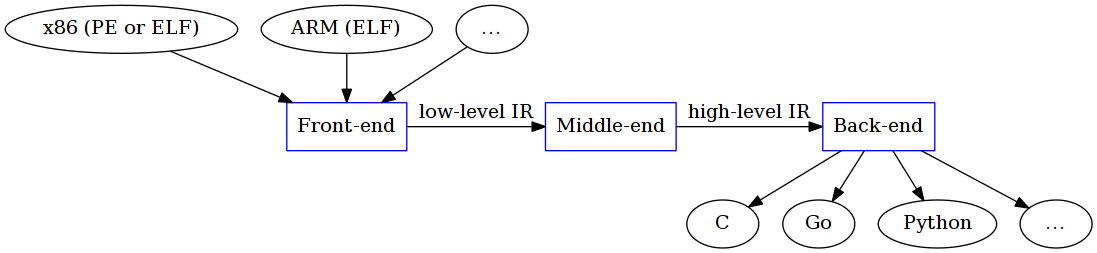
\includegraphics[width=\textwidth]{inc/modules_overview.png}
		\caption{The front-end module accepts several executable file formats (PE, ELF, …) as input and translates their platform dependent assembly (x86, ARM, …) to a low-level IR. The middle-end module then lifts the low-level IR to a high-level IR through a set of decompilation passes. Finally the backend-module translates the high-level IR into one of several target programming languages (C, Go, Python, …).}
		\label{modules_overview}
	\end{center}
\end{figure}

The remainder of this section describes the distinct decompilation phases, most of which have been outlined by Cristina Cifuentes in her influential paper \textit{``Reverse Compilation Techniques''} \cite{rev_comp}.

% ~~~ [ Binary Analysis ] ~~~~~~~~~~~~~~~~~~~~~~~~~~~~~~~~~~~~~~~~~~~~~~~~~~~~~~

\subsubsection{Binary Analysis}

The binary analysis phase is responsible for parsing input files of various binary file formats, such as PE and ELF, and present their content in a uniform manner which preserves the relations between file content, virtual addresses and access permissions.

Lorem ipsum dolor sit amet, consectetur adipiscing elit, sed do eiusmod tempor incididunt ut labore et dolore magna aliqua.

% ~~~ [ Disassembly ] ~~~~~~~~~~~~~~~~~~~~~~~~~~~~~~~~~~~~~~~~~~~~~~~~~~~~~~~~~~

\subsubsection{Disassembly}

% TODO: refer to the syntactic analysis phase in C. Cifuentes.

Lorem ipsum dolor sit amet, consectetur adipiscing elit, sed do eiusmod tempor incididunt ut labore et dolore magna aliqua.

% ~~~ [ Semantic Analysis ] ~~~~~~~~~~~~~~~~~~~~~~~~~~~~~~~~~~~~~~~~~~~~~~~~~~~~

\subsubsection{Semantic Analysis}

Lorem ipsum dolor sit amet, consectetur adipiscing elit, sed do eiusmod tempor incididunt ut labore et dolore magna aliqua.

% ~~~ [ Intermediate Code Generation ] ~~~~~~~~~~~~~~~~~~~~~~~~~~~~~~~~~~~~~~~~~

\subsubsection{Intermediate Code Generation}

Lorem ipsum dolor sit amet, consectetur adipiscing elit, sed do eiusmod tempor incididunt ut labore et dolore magna aliqua.

% ~~~ [ Control Flow Graph Generation ] ~~~~~~~~~~~~~~~~~~~~~~~~~~~~~~~~~~~~~~~~

\subsubsection{Control Flow Graph Generation}

Lorem ipsum dolor sit amet, consectetur adipiscing elit, sed do eiusmod tempor incididunt ut labore et dolore magna aliqua.

% ~~~ [ Data Flow Analysis ] ~~~~~~~~~~~~~~~~~~~~~~~~~~~~~~~~~~~~~~~~~~~~~~~~~~~

\subsubsection{Data Flow Analysis}

Lorem ipsum dolor sit amet, consectetur adipiscing elit, sed do eiusmod tempor incididunt ut labore et dolore magna aliqua.

\cite{type_decomp}

% ~~~ [ Control Flow Analysis ] ~~~~~~~~~~~~~~~~~~~~~~~~~~~~~~~~~~~~~~~~~~~~~~~~

\subsubsection{Control Flow Analysis}

Lorem ipsum dolor sit amet, consectetur adipiscing elit, sed do eiusmod tempor incididunt ut labore et dolore magna aliqua.

% --- [ Evaluation of Intermediate Representations ] ---------------------------

\subsection{Evaluation of Intermediate Representations}

% TODO: Very interesting read about the evaluation of IRs specifically for reverse engineering: An Intermediate Representation for Integrating Reverse Engineering Analyses.

% TODO: Check http://indefinitestudies.org/2009/04/03/a-quick-survey-on-intermediate-representations-for-program-analysis/

Lorem ipsum dolor sit amet, consectetur adipiscing elit, sed do eiusmod tempor incididunt ut labore et dolore magna aliqua.

% ~~~ [ LLVM IR ] ~~~~~~~~~~~~~~~~~~~~~~~~~~~~~~~~~~~~~~~~~~~~~~~~~~~~~~~~~~~~~~

\subsubsection{LLVM IR}

Lorem ipsum dolor sit amet, consectetur adipiscing elit, sed do eiusmod tempor incididunt ut labore et dolore magna aliqua.

% ~~~ [ ELIR ] ~~~~~~~~~~~~~~~~~~~~~~~~~~~~~~~~~~~~~~~~~~~~~~~~~~~~~~~~~~~~~~~~~

\subsubsection{ELIR}

% TODO: Research.
% ref: http://www.eresi-project.org/
% Part of ERESI.
% "ERESI development has restarted as of February 2013"
% Seems dead; no new code in 19 months.

Lorem ipsum dolor sit amet, consectetur adipiscing elit, sed do eiusmod tempor incididunt ut labore et dolore magna aliqua.

% ~~~ [ Hex Rays Microcode ] ~~~~~~~~~~~~~~~~~~~~~~~~~~~~~~~~~~~~~~~~~~~~~~~~~~~

\subsubsection{Hex Rays Microcode}

Lorem ipsum dolor sit amet, consectetur adipiscing elit, sed do eiusmod tempor incididunt ut labore et dolore magna aliqua.

\cite{hexrays}

% ~~~ [ Wire ] ~~~~~~~~~~~~~~~~~~~~~~~~~~~~~~~~~~~~~~~~~~~~~~~~~~~~~~~~~~~~~~~~~

\subsubsection{Wire}

% TODO: Check: Wire - A Formal Intermediate Language for Binary Analysis

Lorem ipsum dolor sit amet, consectetur adipiscing elit, sed do eiusmod tempor incididunt ut labore et dolore magna aliqua.


% ~~~ [ Valgrind IR ] ~~~~~~~~~~~~~~~~~~~~~~~~~~~~~~~~~~~~~~~~~~~~~~~~~~~~~~~~~~

\subsubsection{Valgrind IR}

Lorem ipsum dolor sit amet, consectetur adipiscing elit, sed do eiusmod tempor incididunt ut labore et dolore magna aliqua.

% ~~~ [ QEMU IR ] ~~~~~~~~~~~~~~~~~~~~~~~~~~~~~~~~~~~~~~~~~~~~~~~~~~~~~~~~~~~~~~

\subsubsection{QEMU IR}

Lorem ipsum dolor sit amet, consectetur adipiscing elit, sed do eiusmod tempor incididunt ut labore et dolore magna aliqua.

% ~~~ [ REIL ] ~~~~~~~~~~~~~~~~~~~~~~~~~~~~~~~~~~~~~~~~~~~~~~~~~~~~~~~~~~~~~~~~~

\subsubsection{REIL}

% TODO: Research.
% Check: REIL: A platform-independent intermediate representation of disassembled code for static code analysis
%
% REIL. Used in BinNavi (aquired by Google in 2011), the Reverse Engineering Intermediate Language defines a very simple RISC architecture (17 instructions), with the nice property that each instruction has at most one side-effect.
% lang ref: http://www.zynamics.com/binnavi/manual/html/reil_language.htm
% http://blog.zynamics.com/2010/06/22/the-reil-language-part-ii/


Lorem ipsum dolor sit amet, consectetur adipiscing elit, sed do eiusmod tempor incididunt ut labore et dolore magna aliqua.

% ~~~ [ SAIL ] ~~~~~~~~~~~~~~~~~~~~~~~~~~~~~~~~~~~~~~~~~~~~~~~~~~~~~~~~~~~~~~~~~

\subsubsection{SAIL}

% TODO: Check: SAIL: Static Analysis Intermediate Language with a Two-Level Representation

Lorem ipsum dolor sit amet, consectetur adipiscing elit, sed do eiusmod tempor incididunt ut labore et dolore magna aliqua.

% === [ Related Work ] =========================================================

\section{Related Work}

Lorem ipsum dolor sit amet, consectetur adipiscing elit, sed do eiusmod tempor incididunt ut labore et dolore magna aliqua.

% TODO: Change the structure of this section.
%
% * Native Code to LLVM IR
%    - Dagger
%    - Fracture
%    - MC-Semantics
%       dagger and fracture rely on TableGen for instruction semantics, McSema doesn't.
%    - BAP?
% * Decompilers and Decompilation Frameworks
%    - The dcc Decompiler
%    - The opencl Decompiler
%    - C-Decompiler
%    - The REcompile Decompilation Framework
%    - Boomerang
%    - radare
%    - IDA Hex-Rays
%    - The Retargetable Decompiler

% --- [ Academic Prototypes ] --------------------------------------------------

\subsection{Academic Prototypes}

Lorem ipsum dolor sit amet, consectetur adipiscing elit, sed do eiusmod tempor incididunt ut labore et dolore magna aliqua.

% ~~~ [ The dcc Decompiler ] ~~~~~~~~~~~~~~~~~~~~~~~~~~~~~~~~~~~~~~~~~~~~~~~~~~~

\subsubsection{The \texttt{dcc} Decompiler}

Lorem ipsum dolor sit amet, consectetur adipiscing elit, sed do eiusmod tempor incididunt ut labore et dolore magna aliqua.

\cite{rev_comp}

% ~~~ [ The opencl Decompiler ] ~~~~~~~~~~~~~~~~~~~~~~~~~~~~~~~~~~~~~~~~~~~~~~~~

\subsubsection{The \texttt{opencl} Decompiler}

Lorem ipsum dolor sit amet, consectetur adipiscing elit, sed do eiusmod tempor incididunt ut labore et dolore magna aliqua.

\cite{decomp_llvm}

% ~~~ [ C-Decompiler ] ~~~~~~~~~~~~~~~~~~~~~~~~~~~~~~~~~~~~~~~~~~~~~~~~~~~~~~~~~

\subsubsection{The \texttt{C-Decompiler}}

The \texttt{C-Decompiler} translates machine code into C source code. It focuses primarily on improving the readability of the generated C source code, and does so by extending the traditional decompilation techniques outlined by Cristina Cifuentes in three ways. Firstly, the data flow analysis phase is refined using a shadow stack, which corresponds to a virtual stack capable of tracking stack variables and updates to the stack pointer register. Secondly, the register propagation algorithms are adapted to handle use-def chains across multiple basic blocks. Lastly, library signatures are generated for the C++ Standard Template Library \cite{readable_decomp}.

% ~~~ [ The REcompile Decompilation Framework ] ~~~~~~~~~~~~~~~~~~~~~~~~~~~~~~~~

\subsubsection{The \texttt{REcompile} Decompilation Framework}

Lorem ipsum dolor sit amet, consectetur adipiscing elit, sed do eiusmod tempor incididunt ut labore et dolore magna aliqua.

\cite{recompile}

% --- [ Open Source Projects ] -------------------------------------------------

\subsection{Open Source Projects}

Lorem ipsum dolor sit amet, consectetur adipiscing elit, sed do eiusmod tempor incididunt ut labore et dolore magna aliqua.

% ~~~ [ Boomerang ] ~~~~~~~~~~~~~~~~~~~~~~~~~~~~~~~~~~~~~~~~~~~~~~~~~~~~~~~~~~~~

\subsubsection{Boomerang}

Lorem ipsum dolor sit amet, consectetur adipiscing elit, sed do eiusmod tempor incididunt ut labore et dolore magna aliqua.

\cite{boomerang}

% ~~~ [ radare ] ~~~~~~~~~~~~~~~~~~~~~~~~~~~~~~~~~~~~~~~~~~~~~~~~~~~~~~~~~~~~~~~

\subsubsection{radare}

Lorem ipsum dolor sit amet, consectetur adipiscing elit, sed do eiusmod tempor incididunt ut labore et dolore magna aliqua.

\cite{radare}

% --- [ Commercial Products ] --------------------------------------------------

\subsection{Commercial Products}

Lorem ipsum dolor sit amet, consectetur adipiscing elit, sed do eiusmod tempor incididunt ut labore et dolore magna aliqua.

% TODO: Add section about the Hopper decompiler. ref: http://www.hopperapp.com/

% ~~~ [ Hex-Rays Decompiler ] ~~~~~~~~~~~~~~~~~~~~~~~~~~~~~~~~~~~~~~~~~~~~~~~~~~

\subsubsection{Hex-Rays Decompiler}

Lorem ipsum dolor sit amet, consectetur adipiscing elit, sed do eiusmod tempor incididunt ut labore et dolore magna aliqua.

\cite{hexrays}

% --- [ Decompilation as a Services ] ------------------------------------------

\subsection{Decompilation as a Services}

Lorem ipsum dolor sit amet, consectetur adipiscing elit, sed do eiusmod tempor incididunt ut labore et dolore magna aliqua.

% ~~~ [ The Retargetable Decompiler ] ~~~~~~~~~~~~~~~~~~~~~~~~~~~~~~~~~~~~~~~~~~

\subsubsection{The Retargetable Decompiler}

Lorem ipsum dolor sit amet, consectetur adipiscing elit, sed do eiusmod tempor incididunt ut labore et dolore magna aliqua.

\cite{retargetable_decomp}

%%%%%%%%%%%%%%%%%%%%%%%%%%%%%%%%%%%%%%%%%%%%%%%%%%%%%%%%%%%%%%%%%%%%%%%%%%%%%%%%
% Design and Implementation
%%%%%%%%%%%%%%%%%%%%%%%%%%%%%%%%%%%%%%%%%%%%%%%%%%%%%%%%%%%%%%%%%%%%%%%%%%%%%%%%

% === [ Requirements ] =========================================================

\section{Requirements}

The requirements in this section have been categorized using MoSCoW prioritization \cite{MoSCoW_analysis}, a summary of which is presented in table \ref{MoSCoW_priorities}.

\begin{table}[htbp]
	\begin{center}
		\begin{tabular}{|l|l|}
			\hline
			Priority & Description \\
			\hline
			MUST & An essential requirement that \textit{must} be satisfied. \\
			SHOULD & An important requirement that \textit{should} be satisfied if possible. \\
			COULD & A desirable requirement that \textit{could} be satisfied but it is not necessary. \\
			WON'T & A future requirement that \textit{will not} be satisfied in this release. \\
			\hline
		\end{tabular}
	\end{center}
	\caption{A summary of the MoSCoW (MUST, SHOULD, COULD, WON'T) priorities.}
	\label{MoSCoW_priorities}
\end{table}

% TODO: Cleanup.

\begin{enumerate}
	\item Lexer and parser for the assembly representation of LLVM IR.
	\item Generation of control flow graphs from LLVM IR.
	\item Generation of graph description files (DOT) from control flow graphs.
	\item Create a structured control flow graph using control flow analysis.
	\item Output LLVM IR with information about high-level control structures stored in the basic block names.
	\item \textit{Future ambition}: Output pseudo-code containing the high-level control structures.
\end{enumerate}

\begin{table}[htbp]
	\begin{center}
		\begin{tabular}{|l|l|l|}
			\hline
			Req. ID & Priority & Description and justification \\
			\hline
			\textbf{R1} & MUST & foo. \\
			\hline
		\end{tabular}
	\end{center}
	\caption{foo}
\end{table}


% === [ Methodology ] ==========================================================

\section{Methodology}

Lorem ipsum dolor sit amet, consectetur adipiscing elit, sed do eiusmod tempor incididunt ut labore et dolore magna aliqua.

% TODO: Explain why this specific methodology was chosen, and justify the methods. The justification may be required to be quite detailed, with in-text references.

% --- [ Evolutionary Development and Throwaway Prototyping ] -------------------

\subsection{Evolutionary Development and Throwaway Prototyping}

Lorem ipsum dolor sit amet, consectetur adipiscing elit, sed do eiusmod tempor incididunt ut labore et dolore magna aliqua.

% ~~~ [ Revision Control System ] ~~~~~~~~~~~~~~~~~~~~~~~~~~~~~~~~~~~~~~~~~~~~~~

\subsubsection{Revision Control System}

Lorem ipsum dolor sit amet, consectetur adipiscing elit, sed do eiusmod tempor incididunt ut labore et dolore magna aliqua.

% --- [ Public Issue Tracking ] ------------------------------------------------

\subsection{Public Issue Tracking}

Lorem ipsum dolor sit amet, consectetur adipiscing elit, sed do eiusmod tempor incididunt ut labore et dolore magna aliqua.

% --- [ Continuous Integration ] -----------------------------------------------

\subsection{Continuous Integration}

Lorem ipsum dolor sit amet, consectetur adipiscing elit, sed do eiusmod tempor incididunt ut labore et dolore magna aliqua.

% --- [ Test Driven Design ] ---------------------------------------------------

\subsection{Test Driven Design}

Lorem ipsum dolor sit amet, consectetur adipiscing elit, sed do eiusmod tempor incididunt ut labore et dolore magna aliqua.

% === [ Design ] ===============================================================

\section{Design}

Lorem ipsum dolor sit amet, consectetur adipiscing elit, sed do eiusmod tempor incididunt ut labore et dolore magna aliqua.

% --- [ Choice of Programming Language ] ---------------------------------------

\subsection{Choice of Programming Language}

% TODO: Clarify the benefits and drawbacks of using Go over C++ which would be the obvious choice for LLVM IR heavy projects.

Lorem ipsum dolor sit amet, consectetur adipiscing elit, sed do eiusmod tempor incididunt ut labore et dolore magna aliqua.

% TODO: Mention software composition.

% --- [ Decompiler Pipeline ] --------------------------------------------------

\subsection{Decompiler Pipeline}

% TODO: Describe where the "restructure" component fits in the overall decompilation pipeline. Mention which projects and tools that may be used to fill the gaps.

Lorem ipsum dolor sit amet, consectetur adipiscing elit, sed do eiusmod tempor incididunt ut labore et dolore magna aliqua.

% --- [ System Architecture ] --------------------------------------------------

\subsection{System Architecture}

% TODO: Visualize the dependency graph of the "restructure" tool and describe in detail what input it expects and what output it produces.

Lorem ipsum dolor sit amet, consectetur adipiscing elit, sed do eiusmod tempor incididunt ut labore et dolore magna aliqua.

% TODO: Mention package division.

% === [ Development ] ==========================================================

\section{Development}

% TODO: Brainstorm about which sections are actually relevant and how they should be structured.

Lorem ipsum dolor sit amet, consectetur adipiscing elit, sed do eiusmod tempor incididunt ut labore et dolore magna aliqua.

% --- [ Formal Grammar for a subset of LLVM IR ] -------------------------------

\subsection{Formal Grammar for a subset of LLVM IR}

% TODO: Mention previous (partial but incomplete) work.

Lorem ipsum dolor sit amet, consectetur adipiscing elit, sed do eiusmod tempor incididunt ut labore et dolore magna aliqua.

% --- [ Documentation ] --------------------------------------------------------

\subsection{Documentation}

% TODO: Both API documentation and end user documentation with example use cases (perhaps also covering related projects such as McSema).

Lorem ipsum dolor sit amet, consectetur adipiscing elit, sed do eiusmod tempor incididunt ut labore et dolore magna aliqua.

% --- [ Ideomatic Language Use ] -----------------------------------------------

\subsection{Ideomatic Language Use}

Lorem ipsum dolor sit amet, consectetur adipiscing elit, sed do eiusmod tempor incididunt ut labore et dolore magna aliqua.

% --- [ LLVM IR library ] ------------------------------------------------------

\subsection{LLVM IR library}

Lorem ipsum dolor sit amet, consectetur adipiscing elit, sed do eiusmod tempor incididunt ut labore et dolore magna aliqua.

% --- [ TODO ] -----------------------------------------------------------------

\subsection{TODO}

Lorem ipsum dolor sit amet, consectetur adipiscing elit, sed do eiusmod tempor incididunt ut labore et dolore magna aliqua.

% --- [ Testing ] --------------------------------------------------------------

\subsection{Testing}

Lorem ipsum dolor sit amet, consectetur adipiscing elit, sed do eiusmod tempor incididunt ut labore et dolore magna aliqua.

% ~~~ [ Fuzzing the LLVM IR Parser ] ~~~~~~~~~~~~~~~~~~~~~~~~~~~~~~~~~~~~~~~~~~~

\subsubsection{Fuzzing the LLVM IR Parser}

Lorem ipsum dolor sit amet, consectetur adipiscing elit, sed do eiusmod tempor incididunt ut labore et dolore magna aliqua.

%%%%%%%%%%%%%%%%%%%%%%%%%%%%%%%%%%%%%%%%%%%%%%%%%%%%%%%%%%%%%%%%%%%%%%%%%%%%%%%%
% Evaluation and Conclusion
%%%%%%%%%%%%%%%%%%%%%%%%%%%%%%%%%%%%%%%%%%%%%%%%%%%%%%%%%%%%%%%%%%%%%%%%%%%%%%%%

% === [ Evaluation ] ===========================================================

\section{Evaluation}

Lorem ipsum dolor sit amet, consectetur adipiscing elit, sed do eiusmod tempor incididunt ut labore et dolore magna aliqua.

% --- [ Evaluation against Requirements ] --------------------------------------

\subsection{Evaluation against Requirements}

Lorem ipsum dolor sit amet, consectetur adipiscing elit, sed do eiusmod tempor incididunt ut labore et dolore magna aliqua.

% --- [ TODO ] -----------------------------------------------------------------

\subsection{TODO}

Lorem ipsum dolor sit amet, consectetur adipiscing elit, sed do eiusmod tempor incididunt ut labore et dolore magna aliqua.

% --- [ Third Party Adaptation ] -----------------------------------------------

\subsection{Third Party Adaptation}

Lorem ipsum dolor sit amet, consectetur adipiscing elit, sed do eiusmod tempor incididunt ut labore et dolore magna aliqua.

% --- [ Profiling and Benchmarks ] ---------------------------------------------

\subsection{Profiling and Benchmarks}

Lorem ipsum dolor sit amet, consectetur adipiscing elit, sed do eiusmod tempor incididunt ut labore et dolore magna aliqua.

% === [ Future Work ] ==========================================================

\section{Future Work}

Lorem ipsum dolor sit amet, consectetur adipiscing elit, sed do eiusmod tempor incididunt ut labore et dolore magna aliqua.

% === [ Conclusion ] ===========================================================

\section{Conclusion}

Lorem ipsum dolor sit amet, consectetur adipiscing elit, sed do eiusmod tempor incididunt ut labore et dolore magna aliqua.

% --- [ Introduction ] ---------------------------------------------------------

\subsection{Introduction}

Lorem ipsum dolor sit amet, consectetur adipiscing elit, sed do eiusmod tempor incididunt ut labore et dolore magna aliqua.

% --- [ Project Summary ] ------------------------------------------------------

\subsection{Project Summary}

% TODO: Summarise the key findings of your report. No new information should be included.

Lorem ipsum dolor sit amet, consectetur adipiscing elit, sed do eiusmod tempor incididunt ut labore et dolore magna aliqua.

% --- [ Personal Development ] -------------------------------------------------

\subsection{Personal Development}

Lorem ipsum dolor sit amet, consectetur adipiscing elit, sed do eiusmod tempor incididunt ut labore et dolore magna aliqua.

% --- [ Final Thoughts ] -------------------------------------------------------

\subsection{Final Thoughts}

Lorem ipsum dolor sit amet, consectetur adipiscing elit, sed do eiusmod tempor incididunt ut labore et dolore magna aliqua.

\pagebreak

%%%%%%%%%%%%%%%%%%%%%%%%%%%%%%%%%%%%%%%%%%%%%%%%%%%%%%%%%%%%%%%%%%%%%%%%%%%%%%%%
% References
%%%%%%%%%%%%%%%%%%%%%%%%%%%%%%%%%%%%%%%%%%%%%%%%%%%%%%%%%%%%%%%%%%%%%%%%%%%%%%%%

% === [ References ] ===========================================================

\section{References}

\bibliography{references}

\end{document}
